\documentclass[tikz,border=6pt]{standalone}
\usepackage{pgfplots}
\usepgfplotslibrary{groupplots}
\usetikzlibrary{calc}
\pgfplotsset{compat=1.18}
\begin{document}
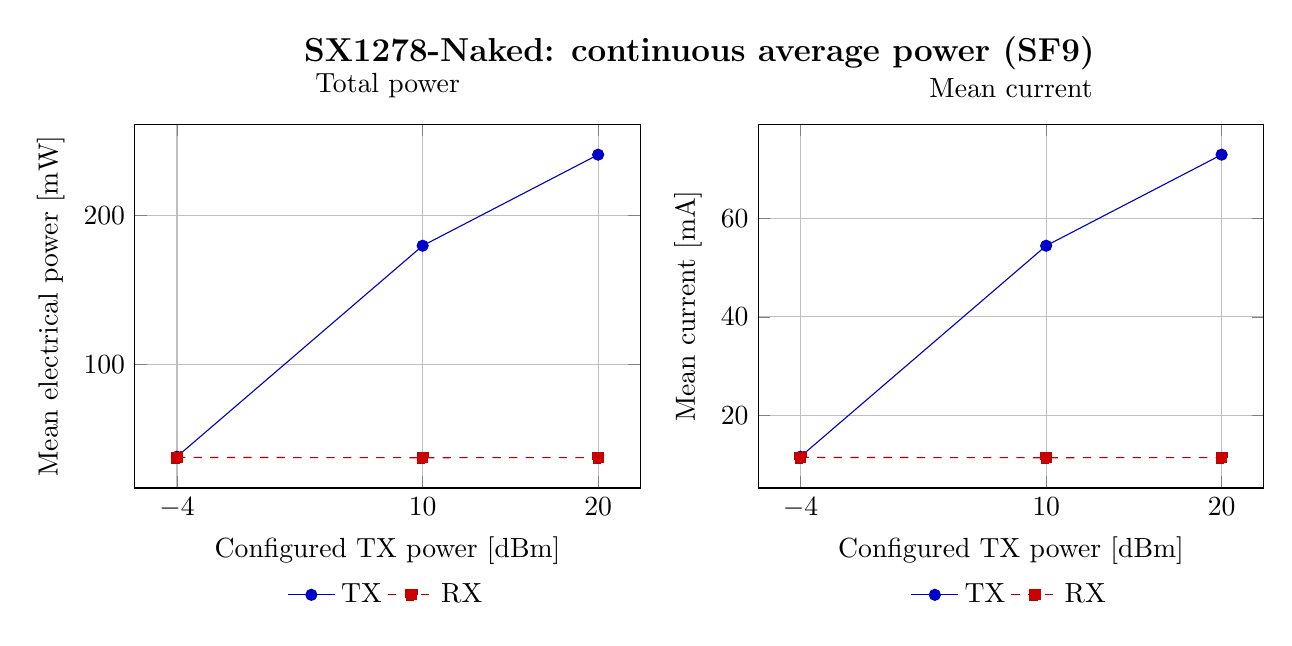
\begin{tikzpicture}
\begin{groupplot}[group style={group size=2 by 1,horizontal sep=1.5cm},width=8cm,height=6.2cm,xtick={-4,10,20},xlabel={Configured TX power [dBm]},grid=both,legend style={draw=none,at={(0.5,-0.23)},anchor=north,legend columns=2}]
\nextgroupplot[title={Total power},ylabel={Mean electrical power [mW]}]
\addplot+[blue!75!black,mark=*] coordinates {(-4,38.3565961) (10,179.644132) (20,240.624636)};\addlegendentry{TX}
\addplot+[red!75!black,dashed,mark=square*] coordinates {(-4,37.8695712) (10,37.6720542) (20,37.7482786)};\addlegendentry{RX}
\nextgroupplot[title={Mean current},ylabel={Mean current [mA]}]
\addplot+[blue!75!black,mark=*] coordinates {(-4,11.6232109) (10,54.4376158) (20,72.9165562)};\addlegendentry{TX}
\addplot+[red!75!black,dashed,mark=square*] coordinates {(-4,11.4756276) (10,11.415774) (20,11.4388723)};\addlegendentry{RX}
\end{groupplot}
\node[font=\bfseries\large] at ($(group c1r1.north)!0.5!(group c2r1.north)+(0,0.9cm)$) {SX1278-Naked: continuous average power (SF9)};
\end{tikzpicture}
\end{document}
